\chapter{Stato dell'arte}
\label{chap:Stato dell'arte}

in questo capitolo presentiamo lo stato dell'arte concernente le tecnologie, i modelli studiati, gli strumenti utilizzati e gli studi su cui questo lavoro si basa. Tratteremo il risparmio energetico, le motivazioni del perché stia diventando un aspetto sempre più importante e i risultati che gli studi hanno prodotto in questi anni, come i sistemi Self-Adaptive basati su vincoli. Successivamente parleremo della tecnologia di comunicazione Bluetooth e nello specifico, presenteremo la sua ultima versione chiamata Low Energy. Illustreremo gli aspetti principali di questa tecnologia, paragonandola alle versioni precedenti, e mostreremo le principali caratteristiche utilizzate in questo lavoro. Successivamente presenteremo la classe di rete Peer-to-Peer, le sue caratteristiche e alcuni modelli di rete appartenenti a questa classe. Tratteremo inoltre, il principio di gossip, gli algoritmi di gossip, la loro classificazione e altri aspetti. Faremo anche alcuni esempi di applicazioni di questi algoritmi e parleremo anche dei alcuni algoritmi di gossip dedicati alle reti Peer-to-Peer. Infine presenteremo gli strumenti di simulazione di reti e protocolli presenti in letteratura, con le loro caratteristiche generali sul sistema di simulazione.

\section{Risparmio energetico}
\subsection{Introduzione}
Nel settore dell'\acf{IT} è ormai da parecchi anni che si guarda al problema dei consumi energetici e alle possibili soluzioni per ridurli. La tendenza verso cui questo settore sta andando è quella di spostare la parte di computazione e di storage sul Web, a carico a grandi aziende che offrono servizi di hosting o clouding. In generale ogni azienda che possiede almeno una server farm medio - grande, si dedica allo studio del risparmio energetico, in quanto la spesa per l'energia per il ramo \acs{IT} non è indifferente ai fini del budget aziendale. Sono stati fatti studi con lo scopo di trovare possibili soluzioni in grado di ridurre gli sprechi. Anche se non ce ne rendiamo conto, nei sistemi \acs{IT} vi sono molti sprechi di energia. In \cite{ranganathan2010-pac} è illustrato che una stima del costo energetico di un Data Center di Google sia nell'ordine dei milioni di dollari per anno e che il consumo energetico del settore \acs{IT} a livello mondiale sia stato stimato attorno ai 40 miliardi di dollari nel 2009. Questo fa capire come con l'evolvere della tecnologia, essa diventi sempre più potente e performante, ma necessiti anche di una quantità maggiore di energia. Per questo motivo le problematiche di consumo energetico, della riduzione degli sprechi e dell'ottimizzazione nell'uso delle risorse sono divenuti sempre più importanti e oggetto di ricerca.

\subsection{Sistemi Self-Adaptative}
In letteratura si trovano molti studi riguardanti possibili soluzioni per una migliore gestione delle risorse e minimizzazione dello spreco di energia. Questi tipi di sistemi si chiamano Self-Adaptative, poiché riescono ad auto regolare parametri interni con l'obiettivo di consumare il minimo quantitativo di energia necessario. In applicazioni reali, bisogna però tenere conto non solo dei vincoli energetici, ma anche della qualità del servizio. E' logico pensare che un'azienda con un data center offra servizi sul web, quindi queste soluzioni self-adaptative devono trovare un compromesso tra consumo di energia e \acf{QoS} da garantire. Questo trade-off è il motivo per cui, al giorno d'oggi, non si sono trovate soluzioni definitive. In letteratura vi sono molti articoli riguardanti sistemi auto adattativi con vincoli di \acs{QoS}, come \cite{PerezMirandolaMers2007-qosbw}, \cite{MarzollaMirandola2013-dpm}, \cite{PerezMirandolaMerseguer2014-relQoSandSWadapt} e \cite{PerezMirandolaMerseguer2014-QoSandPetriNets}. L'idea di base è di poter gestire la quantità di risorse per offrire un determinato servizio, in modo da allocarne il minor numero possibile garantendo allo stesso tempo una qualità del servizio accettabile senza che l'utente ne percepisca un degrado. Questo tipo di adattamento è ovviamente molto dinamico e molto dipendente dalla distribuzione delle richieste che vengono fatte per quel particolare servizio. Ad esempio, in \cite{PerezMirandolaMerseguer2014-QoSandPetriNets} è discussa la situazione di un server mail aziendale ed è presentato su grafico l'utilizzo del server mail nel tempo, nell'arco di una settimana. Dal grafico risulta che tra un giorno e il successivo, quindi di notte, vi è un uso limitato, mentre nella parte diurna dei giorni lavorativi si hanno alti livelli di utilizzo. Nel week-end invece un uso trascurabile. In questo caso tramite un monitoraggio, si può creare un sistema self-adaptive in grado di reagire in anticipo alle variazioni delle richieste in arrivo al server mail, allocando o deallocando risorse preventivamente. Più l'attività che si cerca di studiare non ha una distribuzione di richieste ben definita o è soggetta ad alta variabilità e magari a imprevedibili momenti di burst di richieste, più sarà difficile creare un sistema auto adattativo in grado di reagire preventivamente nel modo corretto. In questo caso lo studio del trade-off è più complicato e bisogna affidarsi a più euristiche. In generale, il concetto è di avere un sistema in grado di allocare solo le risorse necessarie a gestire l'attuale carico di lavoro col minor spreco di energia e garantendo una certa \acs{QoS}. Il sistema deve anche poter anticipare un cambiamento nella frequenza di richieste in ingresso al sistema, allocando o deallocando risorse, sempre con l'obiettivo di avere attive solo le risorse necessarie a gestire il carico di lavoro.

Altri esempi di più recente attualità riguardano il mondo mobile. Dall'avvento dei primi smartphone, gli utenti si sono resi subito conto che uno dei problemi di questi dispositivi è l'eccessivo consumo energetico e la conseguente poca autonomia rispetto ai cellulari della precedente generazione. Infatti, le case produttrici implementano su tutti i loro dispositivi mobili moduli di risparmio energia, in grado di agire sul sistema in base all'impostazione scelta. Anche se le impostazioni variano da brand a brand, in generale si può scegliere tra una modalità normale, senza risparmio energetico, una modalità di semi risparmio energetico e una o due modalità di super risparmio energetico in cui viene disabilitato praticamente ogni tipo di servizio non essenziale, lasciando al dispositivo le sue funzioni core e niente altro. Per quanto riguarda i dispositivi mobili ci si sta muovendo verso il \acf{MCC}, come discusso in \cite{DinhLeeNiyatoWand2013-surveyMCC} . Data la potenza di elaborazione con cui sono equipaggiati i dispositivi mobili oggi giorno, essi sono a tutti gli effetti dei computer in miniatura e quindi possono fare tutto; a prova del sempre crescente numero di applicazioni create e immesse sul mercato. Tutto ciò si traduce in un consumo energetico per sostenere l'esecuzione di tutte queste applicazioni e in un problema d'immagazzinamento dati. Tramite il Mobile Cloud Computing, i dispositivi mobili posso scaricare il peso dell'elaborazione di certi dati e la memorizzazione dei file direttamente nel Cloud, con il risultato di risparmiare fino al 25\% di batteria e molto spazio di memorizzazione.

Un altro ambito in cui è molto importante lo studio e l'ottimizzazione del consumo energetico è quello dell'hardware. Ad esempio nei microprocessori dei computer, ma non solo, sono presenti moduli in grado di monitorare lo stato del chip, la frequenza di lavoro e altri parametri. Nello specifico il modulo \acf{DVS} permette di regolare il voltaggio e quindi la frequenza di lavoro del processore in maniera dinamica, senza dover spegnere il componente. In \cite{MarzollaMirandola2013-dpm} sono presentate le specifiche dell'\acf{ACPI} e proposte come open standard per la gestione della configurazione e dell'energia di sistemi singoli o insieme di sistemi.
\bigskip

 \section{Bluetooth 4.0 Low Energy}
 \label{sec:ble}
 \subsection{Introduzione}
La tecnologia \acf{BLE}, nome in codice Seattle, è una tecnologia wireless ed è stata rilasciata a metà 2010, col rilascio delle le specifiche relative allo standard versione 4.0; ora alla versione 4.2 \cite{BT-CoreSpec4.0} . Dato un sempre maggior impiego dei dispositivi Bluetooth in svariati ambiti come l'IT, moduli di rilevamento e sensori, healtcare \cite{BT-SmartMarks} e altri ancora, questa tecnologia è stata progettata per risolvere uno dei punti deboli delle versioni precedenti: l'alto consumo energetico richiesto. Sulla tecnologia Bluetooth Low Energy, l'associazione Bluetooth SIG lancia la gamma di prodotti denominati Bluetooth Smart identificando una serie di mercati in cui è richiesta una tecnologia a basso consumo energetico come le nascenti strutture delle smart home, healtcare, sport \& fitness. Questa tecnologia è stata progettata e migliorata per tutti questi dispostivi che utilizzano la batteria “a bottone” infatti, alcuni vantaggi presentati dall'azienda sono:
\begin{itemize}
	\item Basso consumo energetico.
	\item Possibile autonomia di mesi o anni per sistemi alimentati da batterie a bottone.
	\item Ampia compatibilità con molti smartphone, computer e tablet.
\end{itemize}
 Sempre nel 2010 si venne a creare un problema di retro compatibilità dei dispositivi Bluetooth Smart con tutti i dispositivi equipaggiati con tecnologie Bluetooth Classic (il Bluetooth Classic è tecnologia dalla versione 1 fino a prima della versione 4). E' risultato che la tecnologia Smart era completamente non compatibile con i dispositivi Bluetooth Classic. Per questo motivo nel 2011 l'azienda cambiò il logo del marchio Bluetooth Smart \cite{BT-Brand}, dividendolo in:
 \begin{itemize}
 	\item Bluetooth Smart.
 	\item Bluetooth Smart Ready.
 \end{itemize}
 L'azienda creò una versione parallela alla Smart, chiamata Smart Ready che implementa l'architettura del Bluetooth 4.0, quindi in grado di comunicare con il Bluetooth sia Smart sia Smart Ready, ma che è anche in grado di comunicare con il Bluetooth Classic, inserendo quell'elemento di retro compatibilità che mancava. Tutti i dispositivi come smartphone, computer e tablet utilizzano tecnologia Bluetooth Smart Ready, mentre dispositivi progettati per funzionare con batterie a bottone o disponibilità energetiche limitate sono equipaggiate solamente con la tecnologia Bluetooth Smart. In figura \ref{fig:bt_01} è rappresentato lo schema di compatibilità, mentre in figura \ref{fig:bt_02} è riportata la tabella di compatibilità pubblicata dall'azienda. 
 
\begin{figure}[t]
	\centering
	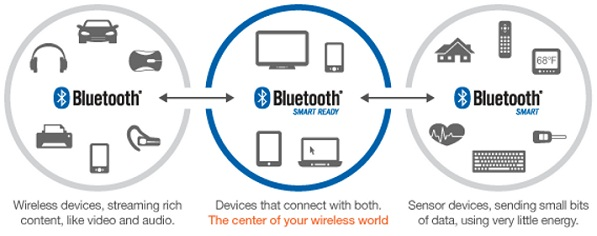
\includegraphics[width=0.9\linewidth, keepaspectratio]{Images/bt/bt_01}
	\caption[Schema di compatibilità.]{Schema di compatibilità tra dispositivi Bluetooth Classic, Smart e Smart Ready \cite{BT-Brand}.}
	\label{fig:bt_01}
\end{figure}

\begin{figure}[t]
	\centering
	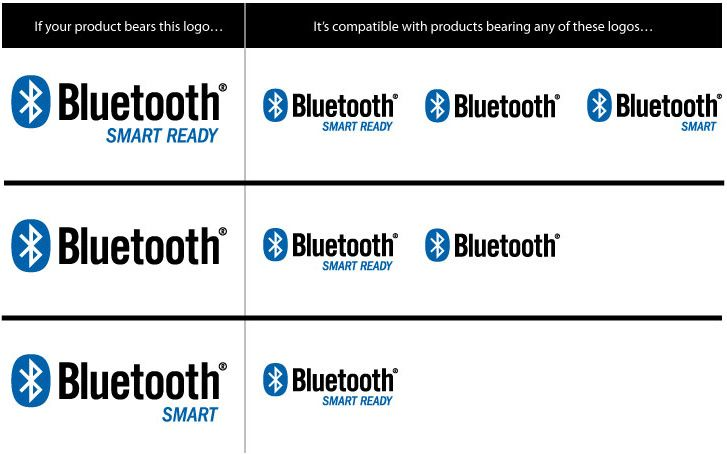
\includegraphics[width=0.9\linewidth, keepaspectratio]{Images/bt/bt_02}
	\caption[Compatibilità tecnologie]{Schema di compatibilità tra tecnologie Bluetooth \cite{BT-2012-tabellacomparativa}.}
	\label{fig:bt_02}
\end{figure}

Tutti gli smartphone, dal 2010 fino ad oggi sono stati equipaggiati con la tecnologia Low Energy Smart Ready. Si è, infatti, costatato un forte incremento nel mercato, di dispositivi che sfruttano tale tecnologia, come i bracciali con tecnologia fitbit, la serie degli i-Watch e gli smartwatch di Android che rendono l'orologio una vera e propria estensione del telefono. Tutti questi dispositivi sfruttano la tecnologia \acs{BLE} rendendo gestibile l'uso di così tante periferiche Bluetooth senza avere drammatiche conseguenze sulla durata delle batterie. Ora l'azienda Bluetooth SIG sta già lavorando a una nuova versione del \acs{BLE}, la versione 4.1. Essa mira a ridurre alcuni conflitti di banda con la tecnologia \acf{LTE}. Infatti, la 4.0 si trova tra le bande 40 e 41 della tecnologia \acs{LTE}. Per risolvere eventuali conflitti, la nuova versione 4.1 effettua un controllo di banda prima di iniziare le trasmissioni. Uno dei primi smatphone a essere equipaggiato con la nuova versione 4.1 del \acs{BLE} è stato il Google Nexus 6.
\bigskip

\subsection{Caratteristiche generali}

In questa sezione presentiamo, alcune caratteristiche del Bluetooth 4.0 Low Energy, anche con qualche comparazione col predecessore Bluetooth Classic per valutare i miglioramenti e i vantaggi che questa nuova tecnologia offre.

\subsubsection{Consumo energia}
La tecnologia \acf{BLE} presenta un consumo ridotto di energia rispetto alla versione precedente, il Bluetooth Classic. Per il Bluetooth Classic vi sono tre classi distinte in cui sono categorizzati i dispositivi, con le relative distanze raggiunte e i consumi associati, mentre per il Bluetooth Low Energy, l'azienda Bluetooth SIG non ha specificato alcun valore massimo di distanza o consumi e quindi il tutto è lasciato come libera scelta ai produttori dei trasmettitori. Questo si traduce ovviamente in una stima per il calcolo del consumo medio di questa nuova tecnologia. Nella \myTab{tab:carBTC} sono riportati i valori di consumi energetici e distanze, relativi al Bluetooth Classic \cite{BT-Basics}, mentre nella \myTab{tab:carBLE} sono riportati i valori di consumo massimo e minimo all'output, per il Bluetooth Low Energy dichiarati nelle specifiche ufficiali \cite{BT-CoreSpec4.0} e il valore stimato medio di distanza raggiungibile presentato in \cite{tesi_tibertoa2013}. Come si può vedere il consumo di energia del Low Energy è ridotto di almeno un ordine di grandezza rispetto al precedente standard Classic.

Come discusso in \cite{sensor2012}, il consumo molto basso da parte del Low Energy, permette a dispositivi alimentati con batterie a bottone, un ciclo di vita che varia tra i 2 giorni e i 14 anni. Inoltre rispetto allo standard Classic, che consente un massimo di 7 dispositivi slave per ogni master, la tecnologia Low Energy offre più flessibilità rendendo questo valore dipendente dall'applicazione e può variare tra 2 e 5.917 slave per master. Riguardo la distanza di trasmissione del \acs{BLE}, è stato stimato essere in media attorno ai 50 metri.
\begin{table}[t]
	\centering
	\footnotesize
	\begin{tabularx}{0.8\textwidth}{lccc}
		\toprule
		&
		\tableheadline{c}{Potenza} &
		\tableheadline{c}{Potenza} &
		\tableheadline{c}{Distanza} \\
		&
		(mW) &
		(dBm) &
		(m) \\
		\midrule
		\tablefirstcol{l}{Classe 1}	& 100 & 20 & \textasciitilde100 \\
		\tablefirstcol{l}{Classe 2}	& 2.5 & 4 & \textasciitilde10 \\
		\tablefirstcol{l}{Classe 3}	& 1 & 0 & \textasciitilde1 \\
		\bottomrule
	\end{tabularx}
	\caption[Bluetooth Classic]{Caratteristiche Bluetooth Classic.}
	\label{tab:carBTC}
\end{table}
%\vskip 3em

\begin{table}[t]
	\centering
	\footnotesize
	\begin{tabularx}{\textwidth}{ccc}
		\toprule
		\tableheadline{c}{Potenza massima} &
		\tableheadline{c}{Potenza mininima} &
		\tableheadline{c}{Distanza} \\
		\midrule
		10 mW (10 dBm) & 0.01 mW (-20 dBm) & \textasciitilde50 m \\
		\bottomrule
	\end{tabularx}
	\caption[Bluetooth Low Energy]{Caratteristiche Bluetooth Low Energy.}
	\label{tab:carBLE}
\end{table}
%\vskip 5em

\subsubsection{Link Layer}
Come descritto nelle specifiche ufficiali del Bluetooth 4.0\cite{BT-CoreSpec4.0}, l'operatività del Link Layer può essere descritta dai seguenti stati:
\begin{itemize}
	\item Stato di Standby.
	\item Stato di Advertising.
	\item Stato di Scanning.
	\item Stato di Initiating.
	\item Stato di Connection.
\end{itemize}
Questi rappresentano i nodi dell'automa a stati finiti che modella il comportamento del Link Layer. Ogni macchina a stati può essere in un solo stato alla volta, ma un Link Layer può avere più istanze di macchina a stati, se il suo hardware lo consente. È necessario però che almeno una delle sue macchine sia in grado di entrare nello stato di Advertising o nello stato di Scanning. Nel caso di macchine a stati multiple, vi sono restrizioni sulle combinazioni possibili di stati attivi tra tutte le macchine a stati; per ulteriori dettagli si può far riferimento alla documentazione ufficiale \cite{BT-CoreSpec4.0}. In figura \ref{fig:bt_fsa} è riportato lo schema della macchina a stati del Link Layer e le relative transizioni tra stati. Di seguito illustriamo il significato di ogni stato:
\begin{figure}[t]
	\centering
	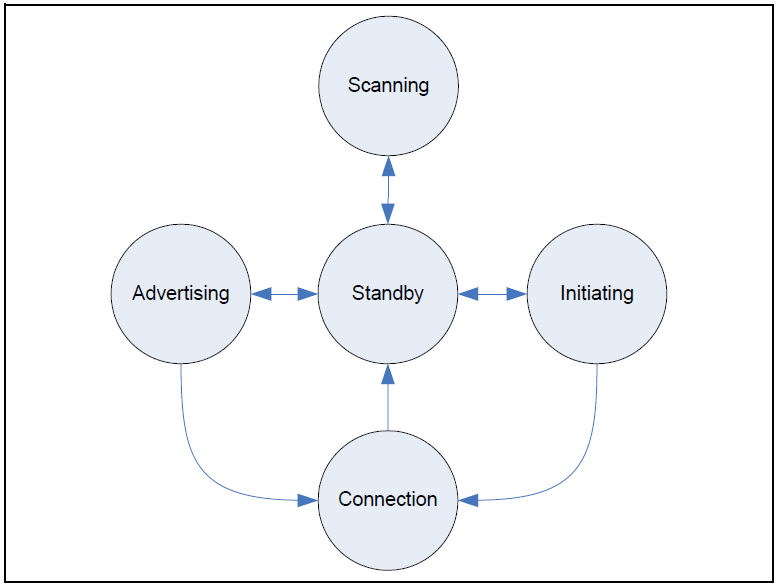
\includegraphics[width=0.9\linewidth, keepaspectratio]{Images/bt/bt_fsa}
	\caption[Link Layer.]{Schema Link Layer BLE\cite{BT-CoreSpec4.0}.}
	\label{fig:bt_fsa}
\end{figure}
\begin{itemize}
	\item \textit{\textbf{Standby}}: è uno stato in cui al dispositivo non è concesso di effettuare alcuna trasmissione o ricezione di pacchetti. Questo stato è raggiungibile da qualsiasi altro stato.
	\item \textbf{\textit{Advertising}}: questo stato permette al dispositivo di  trasmettere pacchetti di advertising e di rimanere in ascolto di eventuali riposte ai pacchetti di advertising che ha inviato. Un dispositivo nello stato di Advertising è chiamato advertiser. Lo stato di Advertising è raggiungibile dallo stato di Standby.
	\item \textbf{\textit{Scanning}}: è uno stato di osservazione. Un dispositivo nello stato di Scanning rimane in ascolto per i pacchetti di advertising e può rispondere, ma mai con l'intenzione di aprire una connessione. Un dispositivo nello stato di Scanning è chiamato scanner e lo stato di Scanning è raggiungibile solo dallo stato di Standby.
	\item \textbf{\textit{Initiating}}: anche questo stato è uno stato di osservazione in cui un dispositivo rimane in ascolto per pacchetti di advertising trasmessi da determinati dispositivi e risponderà a determinati pacchetti se ha l'intenzione di aprire una connessione con quel dispositivo mittente. Un dispositivo in stato di Initiating è chiamato initiator. Lo stato di Initiating è raggiungibile dallo stato di Standby.
	\item \textbf{\textit{Connection}}: questo stato può essere raggiunto sia dallo stato di Advertising sia dallo stato di Initiating. Un dispositivo in stato di Connection, è impegnato in una connessione. Lo stato di Connection si divide a sua volta in due ruoli:
	\begin{itemize}
		\item Ruolo Master.
		\item Ruolo Slave.
	\end{itemize}
	Se lo stato di Connection è raggiunto dallo stato di Advertising si entra col ruolo di Slave, mentre se lo si raggiunge dallo stato di Initiating si entra col ruolo di Master.Un singolo dispositivo col ruolo di Slave può comunicare con un solo Master alla volta.
\end{itemize}

\section{Reti Peer-to-Peer}
\subsection{Introduzione}
La nostra ricerca si è orientata su modelli di reti in grado di rappresentare reti \acf{P2P}, chiamate anche Peer2Peer. Una rete P2P è una rete in cui non vi è una struttura gerarchica e ogni nodo è considerato allo stesso livello di tutti gli altri. Senza la presenza di nodi più importanti o nodi rappresentati centri di conoscenza della rete, nessun nodo può avere una visione completa della rete stessa e non può sapere se la porzione di rete da lui vista rappresenta l'intera rete. Ogni nodo quindi, ha una visione parziale e locale dell'overlay della rete. Le topologie di rete sono rappresentate da grafi bidirezionali, poiché i canali di comunicazione tra i nodi di una rete P2P per le situazioni analizzate, sono bidirezionali. Il modello di rete P2P\cite{peertopeer-book} è un'architettura logica di una rete di nodi paritari, senza alcuna struttura Client-Server predefinita; ogni nodo è paritario a tutti gli altri, infatti, ogni nodo è chiamato peer. La struttura Client-Server è creata solo nel momento della creazione di una connessione tra due nodi, ma più che Client-Server, sarebbe più corretto definirla come Mittente-Destinatario perché non vi sono compiti o azioni predefinite e pre-allocate nelle due parti. Può essere quindi definita una struttura particolare della struttura generica Client-Server.

La principale applicazione di questo modello di rete è stata ed è tuttora quella della condivisione dei file (file sharing), per la quale sono nati tanti sistemi quali Gnutella, FastTrak, Napster, eMule, la rete Torrent, Freenet etc.

Alcune caratteristiche delle reti Peer-to-Peer:
\begin{itemize}
	\item \textit{Basso costo d'implementazione}: non è richiesto l'uso di potenti macchine Server, ma è sufficiente che ogni peer possa sostenere le transazioni dell'utente locale e degli altri peer che vogliono connettersi a lui.
	\item \textit{Amministrazione decentralizzata}: non vi è un server centralizzato di stoccaggio delle informazioni, ma le informazioni sono in possesso dei singoli utenti, localmente, che poi mettono a disposizione della rete.
	\item \textit{Maggiore velocità di trasmissione}: non avendo un Server centralizzato cui tutti i Client si devono connettere per avere un'informazione, causando un calo nella velocità di trasferimento, in un'architettura \acs{P2P} l'informazione può essere reperita anche da più nodi contemporaneamente, infatti, è possibile reperire parti diverse della stessa informazione da nodi diversi e alla fine riassemblare il tutto, col grosso vantaggio di poter avere l'informazione in tempi brevi.
	\item \textit{Sicurezza}: senza la presenza di Server centralizzati, ogni nodo deve garantire per se e per i contenuti che distribuisce, inoltre è anche esposto a ciò che riceve dalla rete che non è controllato da nessuna terza parte. 
\end{itemize}

\subsection{Modelli di Rete}
\label{subsec:modelli_rete}
Poiché abbiamo preso in considerazione l'uso dei grafi, introduciamo due parametri riguardanti i grafi che ne descrivono alcuni aspetti. Essi sono la \textit{edge dependency} e \textit{la degree variance}.
\begin{itemize}
	\item \textbf{\textit{Edge Dependency}}: anche chiamata interdipendenza tra archi. Dato un grafo come in figura \ref{fig:edge_dependency_02}, la edge dependency è definita come la probabilità subordinata che esista un arco tra gli stati S\ped{i}\textasciitilde S\ped{j}, sapendo che esiste un arco tra gli stati S\ped{i}\textasciitilde S\ped{k} e tra S\ped{k}\textasciitilde S\ped{j}. Formalmente, questa probabilità si esprime così P(S\ped{i}\textasciitilde S\ped{j} \textbar\: S\ped{i}\textasciitilde S\ped{k} , S\ped{k}\textasciitilde S\ped{j}) e si può considerare alta se è maggiore della sua probabilità semplice P(S\ped{i}\textasciitilde S\ped{j}).
	\item \textbf{\textit{Degree variance}}: con \textit{degree}(grado) di un nodo si intende il numero di archi incidenti in quel nodo. Un grafo di una rete ha una sua \textit{degree distribution}, la funzione di distribuzione del grado del grafo, da cui si ricava la degree variance che è la varianza della degree distribution. Una degree variance bassa indica un grafo omogeneo in grado. Una degree variance alta è indice della presenza di nodi con molti archi, chiamati \textit{hub}, e di nodi con un pochi archi che rappresentano le foglie del grafo.
\end{itemize}
\begin{figure}[h]
	\centering
	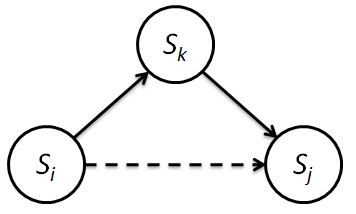
\includegraphics[width=0.5\linewidth,keepaspectratio]{Images/reti/edge_dependency_02}
	\caption[Edge dependency]{Esempio di edge dependency.}
	\label{fig:edge_dependency_02}
\end{figure}
I tre principali modelli di reti presentati in \cite{comparisonGAonRT2012} per la costruzione di reti \acs{P2P} casuali, sono:
\begin{itemize}
	\item Bernoulli Graph.
	\item Random Geometric Graph.
	\item Scale-free Graph.
\end{itemize}
\bigskip

\subsubsection{Bernoulli Graph}
Un Bernoulli Graph $\beta \mathit{\left( N,p_N \right)}$ è un grafo bidirezionale con N nodi nel quale le connessioni hanno una probabilità di esistere pari a $\mathit{p_N}$. Per ogni coppia di nodi vi è una probabilità $\mathit{p_N}$ che il link tra loro esista, indipendentemente da ogni altra connessione. In figura \ref{fig:bernoulli_graph} è riportato un esempio. Un Bernoulli Graph presenta bassa edge dependency e bassa degree variance. Più $\mathit{p_N}$ è alto più il grafo sarà densamente connesso, viceversa più $\mathit{p_N}$ è basso più il grafo sarà poco connesso.
\bigskip
\begin{figure}[h]
	\centering
	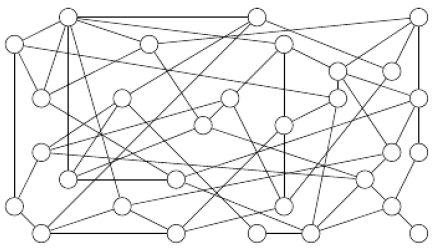
\includegraphics[width=0.7\linewidth,keepaspectratio]{Images/reti/bernoulli_graph}
	\caption[Bernoulli graph]{Esempio di Bernoulli graph\cite{comparisonGAonRT2014-ita}.}
	\label{fig:bernoulli_graph}
\end{figure}
\bigskip

\subsubsection{Random Geometric Graph}
\label{subsubsec:rgg}
Un \acf{RGG} \textit{G(N,$ \rho $)} è un grafo bidirezionale casuale inserito in un'area limitata. Il grafo è generato disponendo in maniera casuale e uniforme gli N nodi all'interno dell'area. Poi due nodi sono connessi se essi tra loro se essi si trovano a una distanza geometrica pari o inferiore a \textit{$ \rho $}. In figura \ref{fig:RandomGeometricGraph} è riportato un esempio. E' facile notare come reti di questo tipo siano estremamente adatte alla rappresentazione di reti wireless, caratterizzate dalla distanza fisica tra i nodi e da un valore soglia \textit{$ \rho $} entro il quale è possibile eseguire trasmissioni. Un \acs{RGG} presenta un'alta edge dependency, dovuta all'importanza della vicinanza fisica tra i nodi, e una bassa degree variance.
\bigskip
\begin{figure}[h]
	\centering
	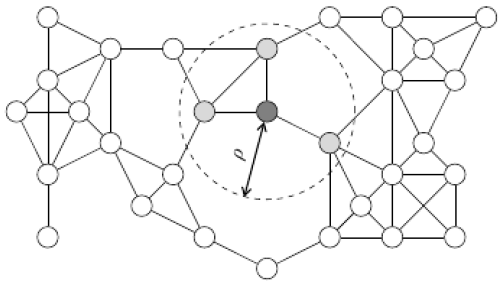
\includegraphics[width=0.7\linewidth,keepaspectratio]{Images/reti/RandomGeometricGraph}
	\caption[Random Geometric grah]{Esempio di Random Geometric graph\cite{comparisonGAonRT2014-ita}.}
	\label{fig:RandomGeometricGraph}
\end{figure}
\bigskip

\subsubsection{Scale-free Graph}
Un Scale-free Graph \textit{S(N,m)} è un grafo bidirezionale con una bassa edge dependency e un'alta degree variance, dovuta alle sue connessioni distribuite secondo legge potenza. Reti di questo tipo sono generate partendo con un insieme di nodi $\mathit{m_0}$, poi a ogni ciclo si aggiunge un nodo e si collegano i suoi $\textit{m}$ archi ad altri nodi già presenti nel grafo. La probabilità che un nuovo nodo sia collegato a un nodo già esistente è proporzionale al grado di quest'ultimo. Collegamenti di questo tipo si dicono preferenziali e fanno si che si creino pochi nodi, chiamati \textit{hub}, con un grado medio alto di circa $\textit{2m}$, e molti nodi chiamati periferici, con grado medio compreso tra $\textit{m}$ e $\textit{2m}$. In figura \ref{fig:scale-free} è riportato un esempio.
\bigskip
\begin{figure}[h]
	\centering
	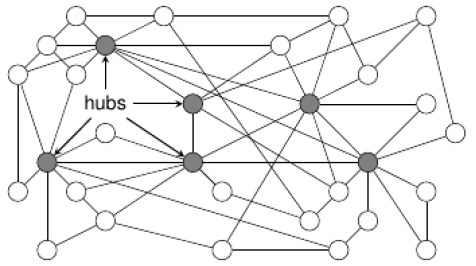
\includegraphics[width=0.7\linewidth,keepaspectratio]{Images/reti/scale-free}
	\caption[Scale-free graph]{Esempio di Scale-free graph\cite{comparisonGAonRT2014-ita}.}
	\label{fig:scale-free}
\end{figure}
%\bigskip
\medskip

\section{Algoritmi di Gossip}
I protocolli Epidemici, o di Gossip, sono paradigmi computazionali e di comunicazione orientati a sistemi distribuiti su larga scala caratterizzati da alta dinamicità. Il metodo più semplice per la diffusione d'informazioni in una rete è effettuare un broadcast cercando di propagare al maggior numero di nodi l'informazione, ma con lo svantaggio di saturare tutti i canali di comunicazione. Per questo motivo i protocolli di gossip utilizzano un approccio probabilistico per la gestione della diffusione dell'informazione attraverso la rete, con lo scopo di massimizzare la diffusione dell'informazione sovraccaricando il meno possibile i canali di comunicazione. In un protocollo epidemico, un nodo che ha un'informazione sceglierà in modo casuale un nodo vicino con cui comunicare e tentare di condividere l'informazione.

Uno dei protocolli epidemici più famoso è “Game of life” \cite{gardner1970-gameoflife}, un automa cellulare sviluppato dal matematico inglese John Conway sul finire degli anni sessanta. L'ambiente per quest'algoritmo è un insieme di celle, dove ogni cella ha 8 celle vicine come mostrato in figura 2.5. Lo scopo dell'algoritmo è di diffondere il seme della vita, quindi ogni cella può essere occupata o no in base alle seguenti regole:
\begin{itemize}
	\item Nascita: se una cella non occupata ha tre celle vicine occupate, diventa anch'essa occupata.
	\item Morte: se una cella occupata ha $0$ o $1$ cella vicina occupata, muore di solitudine, oppure se ha dalle 4 alle 8 celle vicine occupate, muore di sovraffollamento.
	\item Sopravvissuta: se una cella occupata ha $2$ o $3$ celle vicine occupate, essa sopravvive alla generazione successiva.
\end{itemize}

\begin{figure}[bh]
\centering
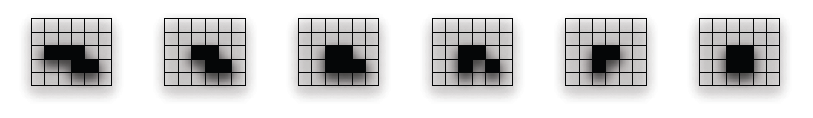
\includegraphics[width=1\linewidth,keepaspectratio]{Images/algoritmi_gossip/game_of_life}
\caption[Game of Life]{Algoritmo Game of Life}
\label{fig:game_of_life}
\end{figure}

\subsection{Classificazione degli algoritmi epidemici}
Come discusso in \cite{schindel2004-epidemicAlg} in ogni algoritmo epidemico c'è sempre un insieme di unità che è chiamato popolazione, che comunicano tra loro. La diffusione di un messaggio deve seguire un insieme specifico di regole. Regole diverse creano la varietà di algoritmi che oggi conosciamo. Qualsiasi sia l'algoritmo però, la cosa importante è che a ogni istante di tempo t o ad ogni iterazione dell'algoritmo, ogni unità della popolazione sia in uno dei seguenti tre stati, riguardo a una specifica informazione:
\begin{itemize}
		\item Suscettible (suscettibile): l'unità non conosce nulla dell'informazione in questione ma è disposta a venirne a conoscenza.
		\item Infected (contagiata): l'unità è a completa conoscenza dell'informazione in questione e utilizza il set di regole per diffondere a sua volta l'informazione.
		\item Removed (Rimossa): l'unità è a completa conoscenza dell'informazione in questione ma non la diffonde.
\end{itemize}
Sulla base delle definizioni appena descritte, possiamo definire diverse classi di algoritmi, in cui è indicato per ogni classe come in generale sono trattate le informazioni. Le principali classi in cui gli algoritmi vengono suddivisi sono:
\begin{itemize}
	\item \acf{SI}.
	\item \acf{SIS}.
	\item \acf{SIR}.
	
\end{itemize}
Esistono anche altre classi che estendono ulteriormente queste classi, aggiungendo alcuni stati intermedi.

In modelli \textbf{\textit{\acf{SI}}} si ha che i nodi possono essere suscettibili a un'informazione e quando ne vengono a conoscenza, diventano contagiati e vi rimangono fintanto che tutta la popolazione non diventa contagiata. Ciò però richiede ulteriori controlli esterni per decidere quando terminare la diffusione dell'informazione.

A differenza del modello \acs{SI}, in quello \textbf{\textit{\acf{SIS}}} un'unità contagiata può decidere di fermare la diffusione dell'informazione prima che tutta la popolazione sia contagiata. Ogni unità rimossa può tornare a essere contagiata se riceve nuovamente l'informazione che aveva smesso di trasmettere e ricominciare a trasmetterla di nuovo finché non perde nuovamente interesse nel farlo.

Il modello \textbf{\textit{\acf{SIR}}} è molto simile al modello \acs{SIS}, con la differenza che un'unità rimossa rimane rimossa per sempre per quella determinata informazione e non potrà più esser contagiata da quell'informazione. Ciò non impedisce che tale unità possa diventare poi suscettibile a nuove informazioni.

\subsection{Medoti di diffusione}
\cite{schindel2004-epidemicAlg} dice che a ogni iterazione di un  algoritmo, tutte le unità della popolazione che devono comunicare con un nodo, esso sia scelto in maniera casuale tra l'intera popolazione. In generale vi sono tre metodi con cui le unità di una popolazione possono diffondere le informazioni ad altre unità:
\begin{itemize}
	\item Push.
	\item Pull.
	\item Push\&Pull.
\end{itemize}
Ogni algoritmo poi,specifica con vincoli più stringenti regole diverse di selezione del destinatario.
\bigskip

\noindent\textbf{\textit{Metodo Push}}\\
Il metodo di Push prevede che i nodi contagiati prendano l'iniziativa di diffondere l'informazione, quindi a ogni istante t, il nodo contagiato sceglie un nodo casuale e prova a contagiarlo, come mostrato in figura \ref{fig:push}. Questa strategia è molto efficace all'inizio della diffusione, quando vi è un alto numero di unità suscettibili e poche contagiate o rimosse, quindi la probabilità che ogni nodo contagiato ha di scegliere un nodo suscettibile è alta. Questa probabilità decresce col passare del tempo perché la quantità di nodi suscettibili diminuisce e il numero di nodi contagiati o rimossi aumenta, rendendo questo metodo poco affidabile nel lungo periodo. Questo metodo non garantisce che tutta la popolazione sia contagiata. Si veda \cite{schindel2004-epidemicAlg} per ulteriori approfondimenti.

\begin{figure}[bh]
	\centering
	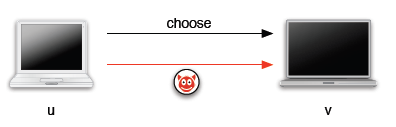
\includegraphics[width=0.6\linewidth,keepaspectratio]{Images/algoritmi_gossip/push}
	\caption[Metodo di Push]{Metodo di Push.}
	\label{fig:push}
\end{figure}
\bigskip


\noindent\textbf{\textit{Metodo Pull}}\\
Il metodo di Pull prevede che un nodo contagiato non si muova attivamente nel diffondere l'informazione, ma che siano i nodi suscettibili a fare richiesta di nuove informazioni ai nodi contagiati. A ogni istante t, un nodo suscettibile seleziona casualmente un altro nodo e gli chiede se ha nuove informazioni. Se il nodo contattato ne ha, allora restituisce l'informazione; in figura \ref{fig:pull} è riportato un esempio. Quest'algoritmo di propagazione è poco efficace all'inizio dell'epidemia perché vi è solo un nodo contagiato e la probabilità di scegliere proprio lui è uno sulla grandezza della popolazione. Col passare del tempo, più l'informazione si diffonde, più alta sarà la probabilità di selezionare un nodo contagiato. Questo metodo non garantisce che il processo di diffusione abbia inizio poiché vi è una probabilità che nessun nodo suscettibile contatti il nodo contagiato, ma vi è anche la possibilità che tutti i nodi scelgano il nodo contagiato generando così un rapido inizio di epidemia. Questo metodo però garantisce che, se l'epidemia inizia, essa si diffonderà a tutta la popolazione. Si veda \cite{schindel2004-epidemicAlg} per ulteriori approfondimenti.

\begin{figure}[h]
	\centering
	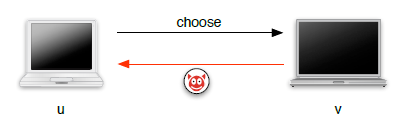
\includegraphics[width=0.6\linewidth,keepaspectratio]{Images/algoritmi_gossip/pull}
	\caption[Metodo di Pull]{Metodo di Pull.}
	\label{fig:pull}
\end{figure}

\noindent\textbf{\textit{Metodo Push\&Pull}}\\
I metodi Push e Pull presentano vantaggi e svantaggi in differenti momenti del processo di diffusione, l'unione dei due ha lo scopo di combinare i vantaggi dei due metodi. In questo caso un nodo contagiato utilizzerà una strategia Push, mentre i nodi suscettibili utilizzeranno un approccio Pull finché non saranno contagiati. Nelle prime fasi della diffusione premierà più la strategià Pulsh, mentre a contagio avanzato si sentirà di più la strategia di Pull. In figura \ref{fig:push_pull} è rappresentato un esempio di strategia Push\&Pull. Si veda \cite{schindel2004-epidemicAlg} per ulteriori approfondimenti.

\begin{figure}[h]
	\centering
	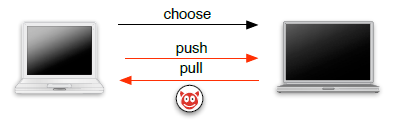
\includegraphics[width=0.6\linewidth,keepaspectratio]{Images/algoritmi_gossip/push_pull}
	\caption[Metodo di Push\&Pull]{Metodo di Push\&Pull.}
	\label{fig:push_pull}
\end{figure}

\subsection{Applicazioni}
Il letteratura vi sono molti esempi di applicazioni degli algoritmi di gossip, tra i tanti citiamo quello per il corretto Replicated Database Maintenance \cite{montresor2004-antiEntropy}, l'Epidemic Routing e il Mantenimento della visione del Network Overlay \cite{montresor2004-overlay}. In merito al Replicated Database Maintenance il primo algoritmo studiato fu il Direct Mail, una soluzione che prevede che il nodo in possesso della nuova informazione debba contattare direttamente ogni altro nodo per diffondere l'aggiornamento. Questo metodo è affidabile perché è molto sensibile allo stato della rete su un unico nodo e sull'unico mittente. Per ovviare a tali problemi sono stati introdotti due principali algoritmi di gossip: Anti-Entropy e il Rumor Mongering. L'Anti-Entropy è un algoritmo di tipo SI, che cerca come dice il nome di contrastare la crescita dell'entropia in un sistema di replicazione dati, facendo si che a ogni ciclo dell'algoritmo, a coppie, i nodi sincronizzino i loro dati. Unico problema è che per la sincronizzazione di database, a volte è necessario trasmettere sulla rete l'intero database. Il Rumor Mongering invece è un algoritmo di tipo SIR che ha lo scopo di propagare tra i nodi solo l'elenco degli aggiornamenti e mai l'intero database. A ogni ciclo ogni nodo che ha la lista aggiornamento non vuota, sceglie un nodo casuale e cerca di propagargli i suoi aggiornamenti. Con questo tipo di algoritmo nasce il problema di trovare un criterio col quale decidere quando smettere di propagare gli aggiornamenti.
 
Da questo sono nati diverse versioni dell'algoritmo di Rumor Mongering, in base ai diversi criteri usati per fermare la propagazione degli aggiornamenti. E' quindi possibile suddividere la classe degli algoritmi di Rumor Mongering nelle seguenti sotto classi:
\begin{itemize}
	\item \textbf{\textit{Blind}}: un nodo contagiato decide di interrompere la diffusione in base al suo stato interno.
	\item \textbf{\textit{Feedbackind}}: un nodo contattato risponde dicendo se già conosce oppure no l'informazione. Il nodo contagiato mittente, in base alla risposta prende una decisione.
	\item \textbf{\textit{Coin}}: il nodo contagiato si fermerà con una probabilità 1/k, dove k è il numero di nodi contattati.
	\item \textbf{\textit{Counter}}: il nodo contagiato incrementa un contatore per ogni informazione inviata con successo. Si ferma quando il contatore supera una soglia prefissata.
\end{itemize}

\subsection{Algoritmi di gossip per il Peer2Peer}
\label{subsec:alg_p2p}
Nel contesto degli algoritmi di gossip relativi a reti \acs{P2P}, presenteremo quelli più utilizzati per la diffusione di messaggi e discussi in \cite{comparisonGAonRT2012} e \cite{comparisonGAonRT2014-ita}. Essi sono il \acf{PB}, \acf{PE} e \acf{FF}. Definiti i seguenti termini:
\begin{itemize}
	\item $ \varLambda_{i} $: insieme di nodi adiacente all'i-esimo nodo.
	\item \textit{V\ped{i}}: la cardinalità di $ \Lambda_{i} $.
	\item \textit{msg}: il messaggio da diffondere.
	\item \textit{p\ped{v},p\ped{e},fanout}: sono i valori probabilistici a ciascun algoritmo, rispettivamente PB,PE e FF.
\end{itemize}
\bigskip

\noindent\textbf{\textit{\acf{PB}}}

Il Probabilistic Broadcast, prevedere che chi ha l'informazione o l'ha ricevuta, la diffonda con una certa probabilità $\mathit{p_v}$ a tutti nodi vicini. La probabilità $\mathit{p_v}$ condiziona in una volta sola, tutto il broadcast; il controllo viene fatto una volta sola per tutto l'insieme dei nodi vicini. L'algoritmo \ref{alg:gossipPB} descrive in pseudo codice il funzionamento di questo metodo.
\bigskip
\begin{algorithm}[h]
	\caption{Probabilistic Broadcast}\label{alg:gossipPB}
	\begin{algorithmic}[1]
		\Function{GossipPB}{msg,\emph{p\ped{v}}}
			\If{Random() $ \leq $ \textit{p\ped{v}}}
				\ForAll{$ \textit{s}_\textit{i} \in \Lambda_{i} $}
					\State Send(msg,\emph{s\ped{j}})
				\EndFor
			\EndIf
		\EndFunction
	\end{algorithmic}
\end{algorithm}
\bigskip

\noindent\textbf{\textit{\acf{PE}}}

Il Probabilistic Edge, prevede che chi ha l'informazione o l'ha ricevuta, la diffonda su ogni arco uscente con una certa probabilità $\mathit{p_e}$ per ogni arco. Rispetto all'algoritmo del \acs{PB}, il controllo viene fatto singolarmente per ogni arco. Il valore di $\mathit{p_e}$ determina se l'algoritmo sia più permissivo o più conservativo in termini di trasmissioni. Lo pseudo codice dell'algoritmo \ref{alg:gossipPE} ne descrive il funzionamento.
\bigskip
\begin{algorithm}[h]
	\caption{Probabilistic Edge}\label{alg:gossipPE}
	\begin{algorithmic}[1]
		\Function{GossipPE}{msg,\emph{p\ped{e}}}
			\ForAll{$ \textit{s}_\textit{j} \in \Lambda_{i} $}
				\If{Random() $ \leq $ \textit{p\ped{e}}}
					\State Send(msg,\emph{s\ped{j}})
				\EndIf
			\EndFor
		\EndFunction
	\end{algorithmic}
\end{algorithm}
\bigskip

\noindent\textbf{\textit{\acf{FF}}}

Il Fixed Fanout, prevedere che chi ha l'informazione o l'ha ricevuta, la diffonda a $\mathit{fanout}$ nodi adiacenti selezionati a caso tra tutti i nodi vicini. Il parametro $\mathit{fanout}$ è definito a priori ed è costante per tutto il tempo dell'esecuzione. A differenza del \acs{PB} e del \acs{PE}, non vi sono fattori di incertezza quindi ad ogni ciclo avremo esattamente $\mathit{fanout}$ trasmissioni. Nel caso il numero di nodi vicini sia inferiore a $\mathit{fanout}$, l'algoritmo prende l'intero insieme di nodi senza scegliere casualmente. L'algoritmo \ref{alg:gossipFF} descrive, tramite pseudo codice, il funzionamento di questo metodo.
\bigskip
\begin{algorithm}[h]
	\caption{Fixed Fanout}\label{alg:gossipFF}
	\begin{algorithmic}[1]
		\Function{GossipPE}{msg,\emph{fanout}}
			\If{$ \textit{fanout} \geq \textit{V}_\textit{i} $}
				\State $ \textit{toSend} \gets \Lambda_i $
			\Else
				\State $ \textit{toSend} \gets \emptyset $
				\For{$ \textit{f} = 1 \;\textbf{to}\; \textit{fanout}$}
					\State random select $ \textit{s}_\textit{j} \in \Lambda_{i}/\textit{toSend} $
					\State $ \textit{toSend} \gets \textit{toSend}\bigcup \textit{s}_\textit{j}$
				\EndFor
			\EndIf
			\ForAll{$ \textit{s}_\textit{j} \in \textit{toSend}$}
				\State Send(msg,\emph{s\ped{j}})
			\EndFor
		\EndFunction
	\end{algorithmic}
\end{algorithm}
\bigskip

\section{Simulatori}
\label{sec:simulatori}
La nostra ricerca si è focalizzata su simulatori di reti Peer-2-Peer, reti in cui tutti i nodi della rete sono allo stesso livello, sono paritetici e non vi è presenza di gerarchie tra nodi, e su simulatori di protocolli basati sia su cicli sia su eventi. In generale simulare qualcosa prevede l'esecuzione di una sequenza di operazioni nel tempo dove le entità che eseguono tali operazioni sono molteplici. Per poter gestire l'esecuzione contemporanea e/o concorrente di più entità il simulatore deve stabilire l'ordine in cui eseguire quale istruzione di quale nodo. La scelta sul come venga stabilito l'ordine di esecuzione caratterizza il motore del simulatore che potrà essere basato su cicli, su eventi o su entrambi. Una simulazione basata su cicli prevede che si definisca uno “time step” di simulazione, che è l'incremento del tempo virtuale di simulazione che definisce la cadenza di ogni ciclo. Tutte le operazioni definite come periodiche verranno eseguite ad ogni ciclo, contemporaneamente. Inoltre qualsiasi evento non periodico che occorre tra un ciclo e un altro verrà schedulato al ciclo successivo. Come si vede in figura \ref{fig:cycled_driven_01}, gli eventi $e_0$, $e_1$ ed $e_2$ accadono tra un ciclo e il successivo, con un passo di simulazione di $\Delta t$. L'evento $e_0$ verrà quindi processato all'instante $\Delta t$, mentre gli eventi $e_1$ ed $e_2$ verranno processati all'instante $4\Delta t$. In questo modo si perde la distribuzione degli eventi, avendo lo scheduler che appiattisce la distribuzione temporale su un unico ciclo, ad ogni iterazione. Questo tipo di simulazioni sono molto vincolanti e non permettono una rappresentazione realistica di una generica classe di nodi. Si adatta molto bene a simulazioni di operazioni batch e/o periodiche. Per poter avere più precisione e dettaglio nella modellazione dell'esecuzione degli eventi vi è lo scheduling guidato dagli eventi che, come dice il nome, ordinerà le operazioni da eseguire in base al momento in cui esse hanno generato o genereranno un evento.

In figura \ref{fig:event_driven_01} è riportato un esempio di scheduling guidato dagli eventi. Il tempo di simulazione non sarà più una progressione costante, ma seguirà il susseguirsi degli eventi, nell'ordine in cui essi avvengono. In questo caso la simulazione avrà inizio con l'evento $e_0$, poi il simulatore salterà all'instante di tempo t1 in quanto lo scheduler prima di $t_1$ non ha nessuna operazione che deve essere eseguita.

\begin{figure}[t]
	\centering
	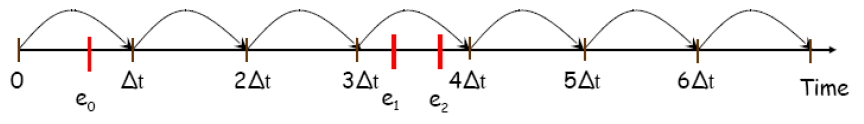
\includegraphics[width=0.9\linewidth, keepaspectratio]{Images/simulatori/cycled_driven_01}
	\caption[Cycle driven scheduling]{Scheduling guidato dai cicli.}
	\label{fig:cycled_driven_01}
\end{figure}

\begin{figure}[t]
	\centering
	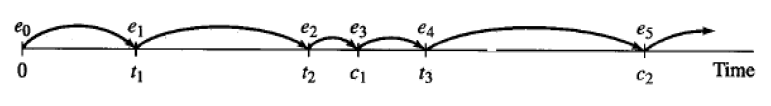
\includegraphics[width=0.9\linewidth, keepaspectratio]{Images/simulatori/event_driven_01}
	\caption[Event driven scheduling]{Scheduling guidato dagli eventi.}
	\label{fig:event_driven_01}
\end{figure}

All'istante $t_1$ avviene l'evento $e_1$ e viene processato, poi si passerà all'istante di tempo $t_2$ perché l'evento $e_2$ è previsto che avvenga in quell'istante e così via tutti gli altri. In generale gli eventi sono relativi per esempio alla ricezione di un messaggio da parte di un nodo. In figura \ref{fig:event_driven_01} vediamo che vi sono gli eventi $e_3$ ed $e_5$ che sono schedulati agli istanti di tempo $c_1$ e $c_2$. Questo è un esempio di integrazione di eventi ciclici in un ambiente guidato dagli eventi. Gli eventi $e_3$ ed $e_5$ sono azioni periodiche e quindi devono essere eseguite ogni “time step” specificato, ma come fare se non vi è un “time step” di simulazione? Il simulatore genererà un evento ogni “time step” di tempo di simulazione associando come evento l'azione periodica. Ciò garantisce di poter avere con un unico motore di scheduling, sia eventi aperiodici che azioni periodiche. In questo caso abbiamo un simulatore basato sia sugli eventi sia sui cicli.

In letteratura esistono tanti simulatori di reti come Mosquite\footnote{\url{http://www.mesquite.com/}} che è una libreria per CSIM, PADS\footnote{\url{http://pads.cs.unibo.it/doku.php?id=start/}} sviluppato dal Dipartimento di Ingegneria Informatica dell'Università di Bologna in grado di simulare protocolli complessi su reti di larga scala o senza una ben definita struttura. Vi è anche PeerSim\footnote{\url{http://peersim.sourceforge.net/}} una libreria Java che fornisce gli strumenti di simulazione basata sia su cicli sia su eventi. Abbiamo poi concentato la nostra attenzione su OMNeT++\footnote{\url{http://omnetpp.org/}}, un framework costruito sulla piattaforma Eclipse\footnote{\url{https://eclipse.org/}} ma scritto in C++. OMNeT++ è uno simulatore basato solo su eventi ma dato il suo intenso sviluppo in ambito commerciale, vi sono disponibili diverse librerie e tool in grado di offrire molte funzionalità di simulazione di protocolli di rete e diverse tipologie di reti. Nel seguito presenteremo brevemente le caratteristiche di PeerSime e OMNeT++.

\subsection{PeerSim}
PeerSim è un software sviluppato in ambiente accademico che consente di simulare reti con una alta flessibilità sul numero di nodi che compongono la rete, rendendolo quindi adatto a simulare reti di grandi dimensioni. In letteratura troviamo diversi riferimenti e trattazioni in merito a questo software, come \cite{montresor2010-peersim}, \cite{montresor2009-peersim_scalabile} e \cite{montresor2009-peersimP2P}. PeerSim poi necessita che venga definito lo stack di protocolli che ogni nodo della rete implementerà; infatti la logica con cui questo simulatore costruisce la rete da simulare è quella di istanziare solo un nodo e poi esso viene copiato, o clonato, tante volte fino a raggiungere il numero di nodi nella rete. Per questo motivo si nota subito  che PeerSim è uno strumento ottimizzato per la simulazione di reti anche di grandi dimensioni e soprattutto, come si può dedurre dal nome, reti soprattutto Peer-to-Peer \cite{montresor2009-peersimP2P}. Non presenta alcun tipo di strumento grafico per la rappresentazione della rete o dei pacchetti in transito tra i nodi, la simulazione è solo computazione e stampa messaggi su console. Vi è la possibilità di utilizzare o estendere alcune funzioni di alcuni componenti del sistema di simulazione che permettono di stampare su file di testo le coordinate dei nodi della rete e/o i rami del grafo della rete nel formato usato da GNUplot\footnote{\url{http://www.gnuplot.info/}} e quindi poi visualizzare il layout di rete. PeerSim necessita che l'utente definisca in un apposito file di configurazione le specifiche di simulazione, della rete, dei protocolli implementati sui nodi, delle dipendenze tra i protocolli. Richiede inoltre di specificare i componenti di inizializzazione, i componenti di controllo e i componenti di osservazione. I componenti di inizializzazione sono componenti che il simulatore eseguirà solo all'inizio del processo di simulazione e hanno il compito di inizializzare i nodi della rete e la rete stessa, ad esempio per stabilire le connessioni tra i nodi. I componenti di controllo sono “agenti” che vengono eseguiti ciclicamente e hanno il compito di agire sulla rete durante la simulazione, per introdurre dinamicità nella stessa come per esempio accendere o spegnere nodi o canali di trasmissione per simulare malfunzionamenti oppure aggiungere o togliere nodi e collegamenti. Questi componenti di controllo sono opzionali. Infine i componenti di osservazione detti anche osservatori sono componenti che operano alla fine della simulazione oppure ciclicamente se resi cycle-based impostando il loro time step. Il loro compito è quello appunto di osservare la rete e permettere di raccogliere dati per analisi. I dati da raccogliere devono essere specificati dall'utente nell'apposita funzione di osservazione che viene eseguita dal motore di simulazione. Un esempio di osservatore è il componente che permette di scrivere su file il layout della rete in formato compatibile con GNUplot. Punto forte di questo simulatore quindi sono la flessibilità sul numero di nodi della rete, le ottime prestazioni di simulazione anche per grandi reti e la scelta di lasciare all'utente l'estensione dei componenti che governano la simulazione.
\bigskip

\subsection{OMNeT++}
OMNeT++ è un framework e libreria di simulazione basata sul linguaggio C++, estendibile e modulare. OMNeT++ è un software di simulazione molto diffuso sia nel settore commerciale sia nel settore scientifico per la simulazione di reti e protocolli di trasmissione, disponibile dal 1997. OMNeT++ è un software che offre un editor di sviluppo basato su Eclipse. Sono disponibili una gran varietà di strutture base come reti wired e wireless ed è possibile aggiungere estensioni che permettono di ampliare la gamma di reti supportate. INET è una delle estensioni più corpose del framework e contiene una grossa quantità di reti e protocolli delle più diffuse strutture di rete utilizzate. Vi sono molte trattazioni in letteratura riguardo a questo strumento, come \cite{omnet2010-book}, \cite{omnet2002-overview} fino a uno studio per uso didattico \cite{omnet2002-edu}.

OMNeT++ è un simulatore di eventi discreti, ma come spiegato all'inizio di questa sezione, è possibile coprire anche situazioni di esecuzione di azioni periodiche, organizzandole come eventi programmati. OMNeT++ contiene anche un ambiente grafico \cite{omnet2002-overview}, Tkenv, per la rappresentazione grafica della struttura della rete e degli eventuali link fisici tra i nodi; è in grado inoltre di eseguire un ri-ordinamento spaziale dei nodi della rete con l'obiettivo di rappresentare il grafico della rete col minor numero di intersezioni tra i collegamenti possibili, per rendere più leggibili lo schema ed eventuali animazioni date dalla simulazione. In \myFig{fig:tkenv_01} è riportato un esempio.
\begin{figure}[tb]
\centering
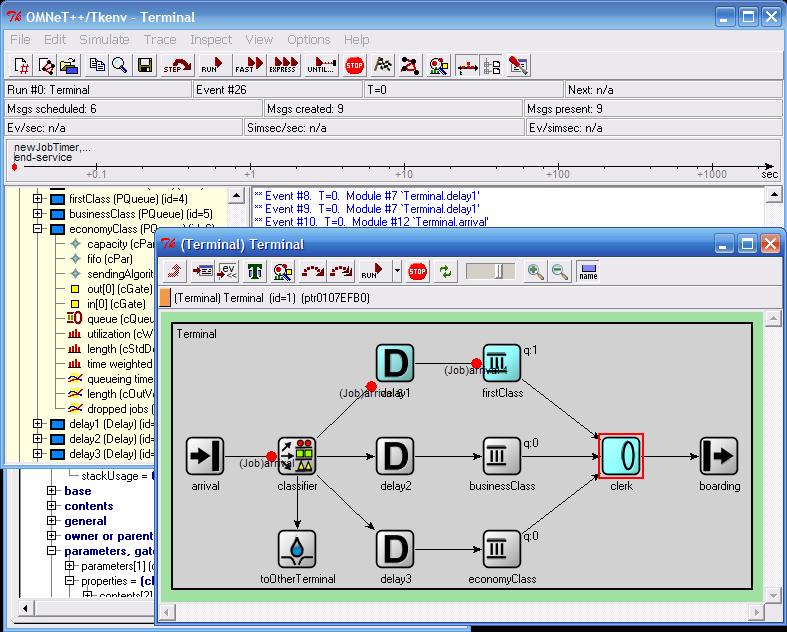
\includegraphics[width=0.7\linewidth]{Images/omnet/tkenv_01}
\caption[tkenv]{Esempio di rappresentazione tramite Tkenv.}
\label{fig:tkenv_01}
\end{figure}
OMNeT++ offre una architettura modulare, cercando di perseguire il principio di riutilizzo dei moduli\cite{omnet2002-overview}. Ogni modulo corrisponde ad un singolo componente della rete o a un componente aggregato, composto a suoa volta da componenti singoli. In questo modo è possibile costruire reti su più livelli, e poter analizzare la rete da punti di vista di diverse granularità. Il linguaggio di alto livello utilizzato per descrivere i moduli si chiama \acf{NED}. La struttura è definita in linguaggio \acs{NED}, mentre il comportamento dei moduli e dei componenti è scritto utilizzando sempre il C++, nei rispettivi file. 
Con OMNeT++, come per PeerSim,  è possibile specificare in appositi file di inizializzazione una lista di parametri necessari a configurare la rete durante la sua fase di inizializzazione prima di iniziare la simulazione vera e propria.  In un singolo file di inizializzazione è possibile specificare più scenari di esecuzione e per ognuno specificare quindi valori diversi. I parametri specificati possono essere letti dal file di Network Definition e usati per creare e impostare la rete secondo i parametri specificati dall'utente nel file di inizializzazione. Tramite il file di Network Definition si può propagare la lettura dei parametri fino ai file C++ con le procedure che modellano il comportamento del componente.
OMNeT++ offre anche un sistema di raccolta dati, tramite il quale si possono poi analizzare i dati raccolti, filtrarli e ottenere differenti rappresentazioni grafiche dei dati stessi \cite{omnet2002-overview}. La raccolta dati può essere sia la sequenza temporale dei risultati, sia una raccolta delle statistiche su dati specifici oppure entrambe le cose.
 \bigskip
 
\subsubsection{File di Inizializzazione}
Un file di inizializzazione è un file necessario alla corretta configurazione della rete, dei suoi componenti e dell'ambiente di simulazione. Un file di inizializzazione ha estensione “.ini” e per comodità verrà anche chiamato “INI file”. In un file di inizializzazione è possibile fornire parametri organizzati in una struttura ad albero, in cui ogni ramo  è uno scenario di simulazione indipendente dagli altri ma eredita tutti i parametri coi rispettivi valori, se non vengono ridefiniti, dello scenario padre. Al momento della simulazione vera e propria, il sistema chiederà all'utente di scegliere quale scenario di simulazione utilizzare se non ve ne è uno specificato direttamente nello script che lancia l'esecuzione di simulazione. 
Nella figura \ref{fig:ini_file} sono riportati due esempi di file d'inizializzazione. Vediamo nella figura \ref{subfig-1:tictoc_ini_01} come sotto la sezione “General” vengano specificati tutti i parametri comuni a tutte le configurazioni e di seguito vengono specificate tutte le altre configurazioni coi parametri specifici per quelle simulazioni. Mentre nella figura \ref{subfig-2:tictoc_ini_02} è riportata una possibile struttura ad albero delle configurazioni.

\begin{figure}[t]
	\subfloat[\label{subfig-1:tictoc_ini_01}]{%
		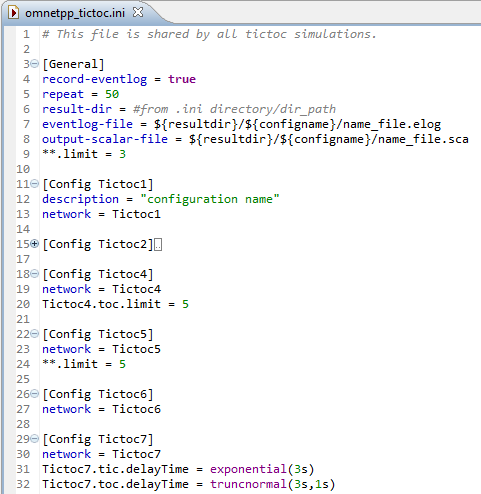
\includegraphics[width=0.45\textwidth, keepaspectratio]{Images/omnet/tictoc_ini_01}
	}
	\hfill
	\subfloat[\label{subfig-2:tictoc_ini_02}]{%
		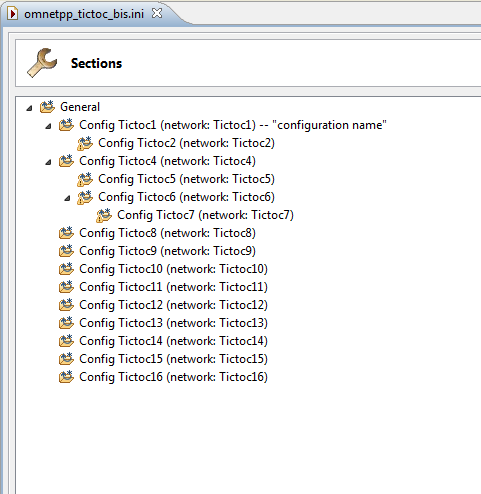
\includegraphics[width=0.45\textwidth, keepaspectratio]{Images/omnet/tictoc_ini_02}
	}
	\caption{Esempio di file di inizializzazione.}
	\label{fig:ini_file}
\end{figure}

In generale ogni file di inizializzazione caratterizza un set di scenari da simulare, quindi si tende a includere nella sezione “General” anche tutti i parametri che servono a impostare correttamente la simulazione o la gestione del framework quali, per esempio l'unità di misura con la quale viene scandito il tempo di simulazione, il numero di ripetizioni per ogni caso di studio che si desidera fare, le varie directory in cui si vogliono salvare i risultati o i dati raccolti.

\subsubsection{Linguaggio NED}
OMNeT++ offre, tramite un linguaggio ad alto livello chiamato Network Definition, la possibilità di definire il layout della rete e la struttura dei singoli componenti e della composizione dei componenti più grandi. Il linguaggio di Network Definition viene usato per creare file di specifica con estensione “.ned”, che abbrevieremo con NED file. Il linguaggio NED è stato pensato per poter implementare singoli moduli in maniera indipendente dall'ambiente, rendendo così facile il loro riutilizzo o estensione. Il sistema ci offre due visibilità del layout di rete ad alto livello: Design e Source. Con la vista Design viene fornita una rappresentazione grafica della rete, se pur sempre ad alto livello, mentre la vista Source permette di vedere e implementare il file come puro codice sorgente. In \myFig{subfig-1:tictoc_ned_01} è riportato un esempio di NED file in vista Design, dove il sistema dice che nel file in questione sono stati usati componenti di tipo “Txc11”, i canali di comunicazioni utilizzati sono dei “Channel” e la rete si può riassumere come un vettore di nodi collegati tra di essi tramite diversi “Channel”. La vera rappresentazione del layout di rete viene fatta solo a runtime in fase di simulazione nel caso venga utilizzato lo strumento grafico Tkenv. In figura \myFig{subfig-2:tictoc_ned_02} invece è riportato lo stesso file della \myFig{subfig-1:tictoc_ned_01} ma in vista Source. Come si può vedere nella figura \myFig{subfig-2:tictoc_ned_02}, in vista sorgente possiamo vedere tutto il codice corrispondente alla vista Design. Si nota che nella prima parte viene definito il singolo componente “Txc11”, poi viene definita la rete come un vettore di componenti “Txc11” e tra essi vi sono dei collegamenti di tipo “Channel”, che è definito dentro la rete.
\bigskip
\begin{figure}[t]
	\subfloat[Vista Design.\label{subfig-1:tictoc_ned_01}]{%
		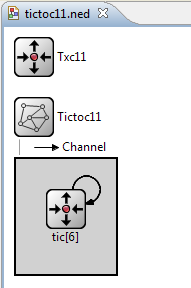
\includegraphics[width=0.38\textwidth, keepaspectratio]{Images/omnet/tictoc_ned_01}
	}
	\hfill
	\subfloat[Vista Source.\label{subfig-2:tictoc_ned_02}]{%
		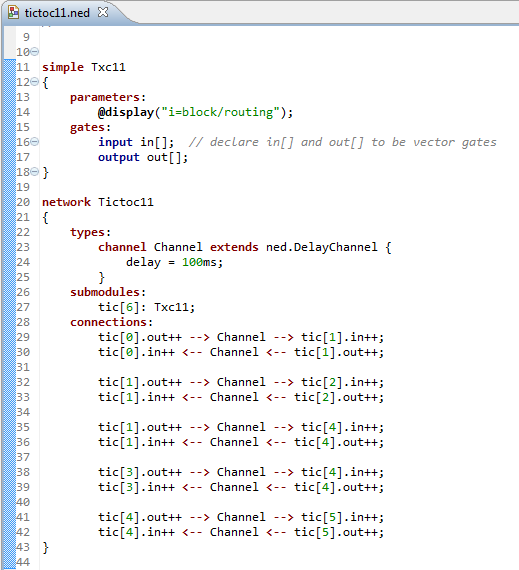
\includegraphics[width=0.52\textwidth, keepaspectratio]{Images/omnet/tictoc_ned_02}
	}
	\caption{Esempio di file NED.}
	\label{fig:ned_file}
\end{figure}
\bigskip

\subsubsection{Raccolta Dati}
OMNeT++ fornisce metodi per la raccolta di dati e statistiche e la possibilità di analizzarli al termine della simulazione. Si possono raccogliere due categorie di dati: i log temporali, chiamati anche event-log e i dati relativi a statistiche. I log temporali non sono altro che rappresentazioni grafiche della successione degli eventi tra i nodi della rete. Molto utile per analizzare la sequenza temporale degli eventi, la loro durata e le loro interazioni, soprattutto quando si hanno parecchi eventi che avvengono in contemporanea; in figura \ref{subfig-1:elog_02} è riportato uno frammento di un event-log. Per quanto riguarda le statistiche, si possono raccogliere dati con riferimento temporale, chiamati vettori, oppure statistiche su dati, chiamati scalari, quali media, varianza, deviazione standard, somma, minimo, massimo e altri ancora. Sia sui vettori che sugli scalari è possibile poi fare delle operazioni di manipolazione dati, come eseguire raggruppamenti, applicare filtri, applicare operazioni ai dati o a gruppi di dati come l'operatore media. Si può applicare l'operatore media a un grafico temporale di vettori, per ottenere l'andamento medio, utile per visualizzare il comportamento asintotico del sistema; in figura \ref{subfig-2:esempio_anf_01} è riportato un esempio. In figura \ref{subfig-3:esempio_anf_grafico_01} è riportato un esempio di rappresentazione grafica di vettori temporali più la rappresentazione dell'andamento medio. In figura \ref{subfig-4:tictoc_scalar_01} invece è riportato un esempio di istogramma come rappresentazione della distribuzione del conteggio di hop necessari per raggiungere hostess destinatario.
\bigskip
%
%\begin{figure}[!h]
%	\centering
%	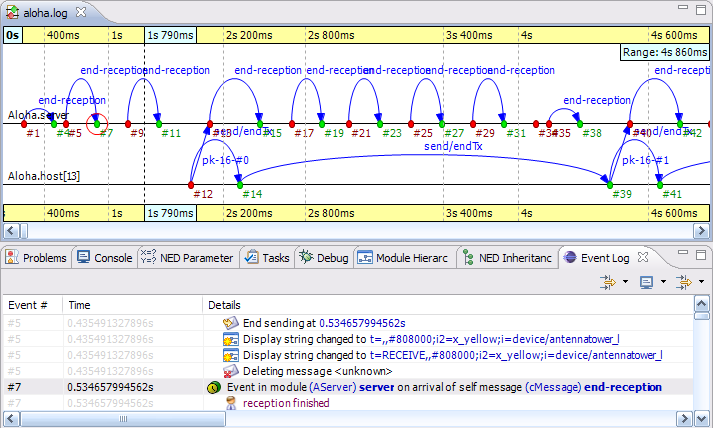
\includegraphics[width=0.7\linewidth]{Images/omnet/elog_02}
%	\caption[anf file]{Esempio di event-log\cite{omnet2002-overview}.}
%	\label{fig:elog_02}
%\end{figure}
%\begin{figure}[!h]
%	\centering
%	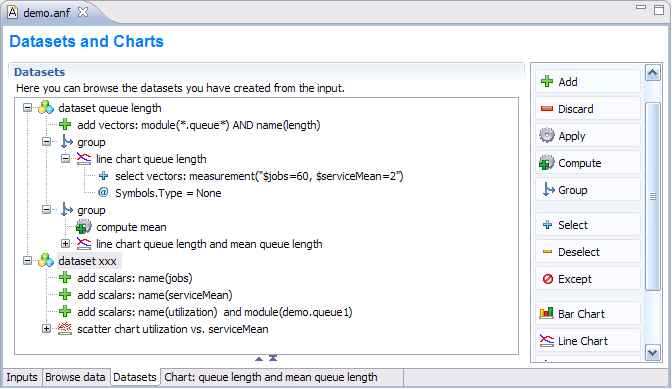
\includegraphics[width=0.7\linewidth]{Images/omnet/esempio_anf_01}
%	\caption[anf file]{Esempio di manipolazione dati\cite{omnet2002-overview}.}
%	\label{fig:esempio_anf_01}
%\end{figure}
%\begin{figure}[!h]
%	\centering
%	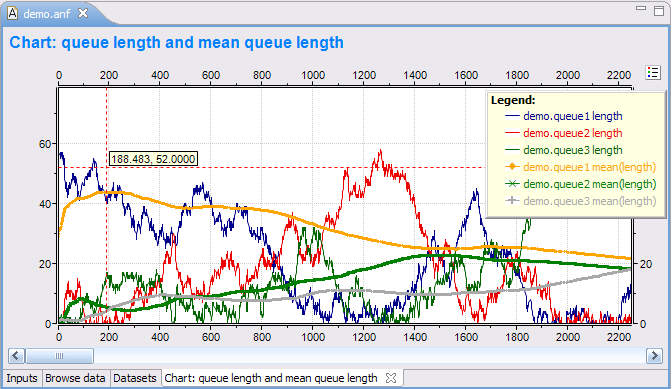
\includegraphics[width=0.7\linewidth]{Images/omnet/esempio_anf_grafico_01}
%	\caption[anf file]{Esempio di grafico temporale di vettori e medi\cite{omnet2002-overview}.}
%	\label{fig:esempio_anf_grafico_01}
%\end{figure}
%\begin{figure}[!h]
%	\centering
%	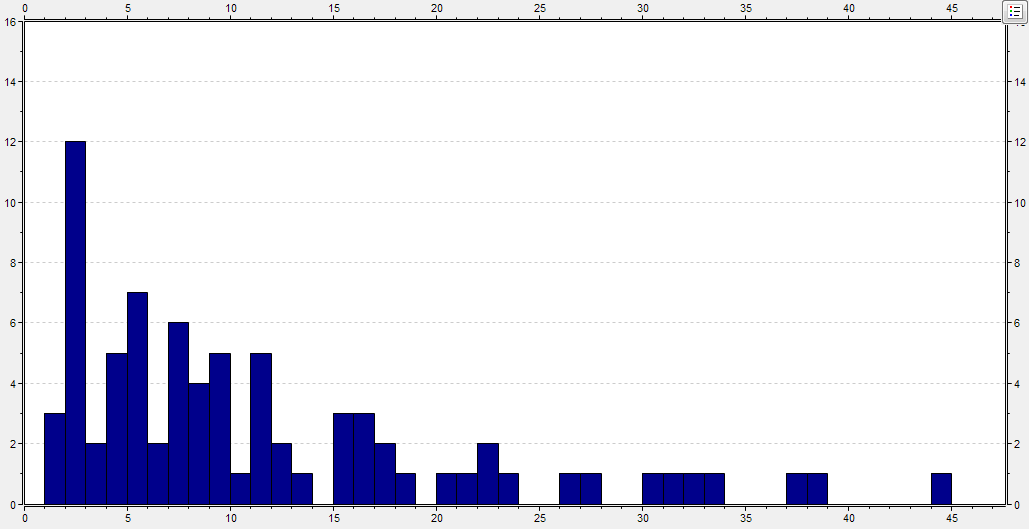
\includegraphics[width=0.7\linewidth]{Images/omnet/tictoc_scalar_01}
%	\caption[anf file]{Esempio di istogramma, grafico per dati scalari\cite{omnet2002-overview}.}
%	\label{fig:tictoc_scalar_01}
%\end{figure}

\begin{figure}[t]
	\subfloat[Esempio di event log\cite{omnet2002-overview}.\label{subfig-1:elog_02}]{%
		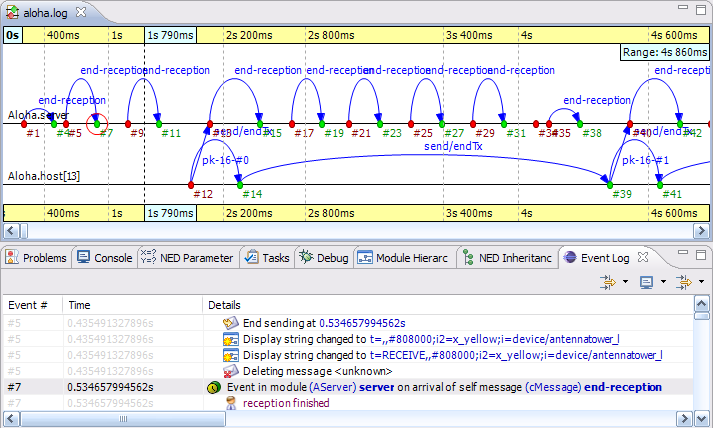
\includegraphics[width=0.45\textwidth, keepaspectratio]{Images/omnet/elog_02}
	}
	\hfill
	\subfloat[Esempio di manipolazione dati\cite{omnet2002-overview}.\label{subfig-2:esempio_anf_01}]{%
		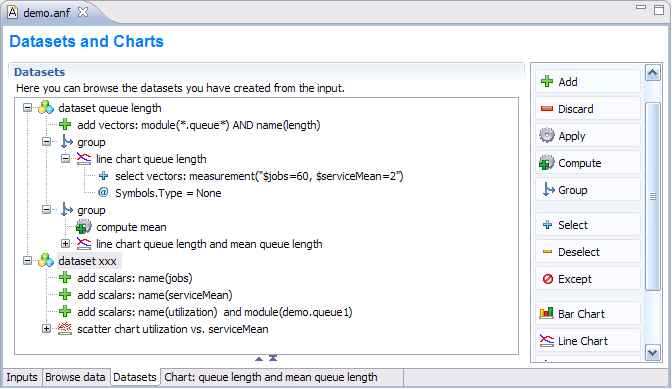
\includegraphics[width=0.45\textwidth, keepaspectratio]{Images/omnet/esempio_anf_01}
	}
	\\
	\subfloat[Esempio di gradico temporale\cite{omnet2002-overview}.\label{subfig-3:esempio_anf_grafico_01}]{%
		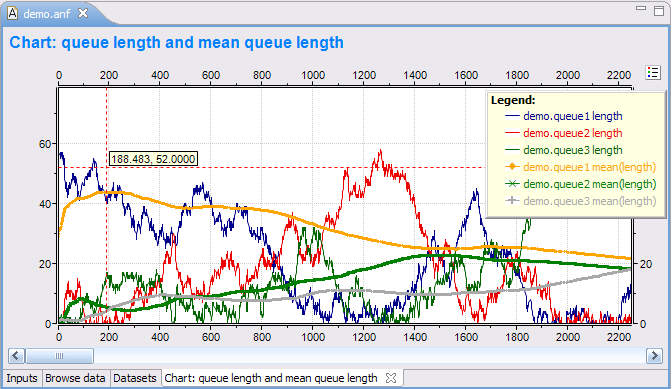
\includegraphics[width=0.45\textwidth, keepaspectratio]{Images/omnet/esempio_anf_grafico_01}
	}
	\hfill
	\subfloat[Esemprio di grafico per scalar, istogramma\cite{omnet2002-overview}.\label{subfig-4:tictoc_scalar_01}]{%
		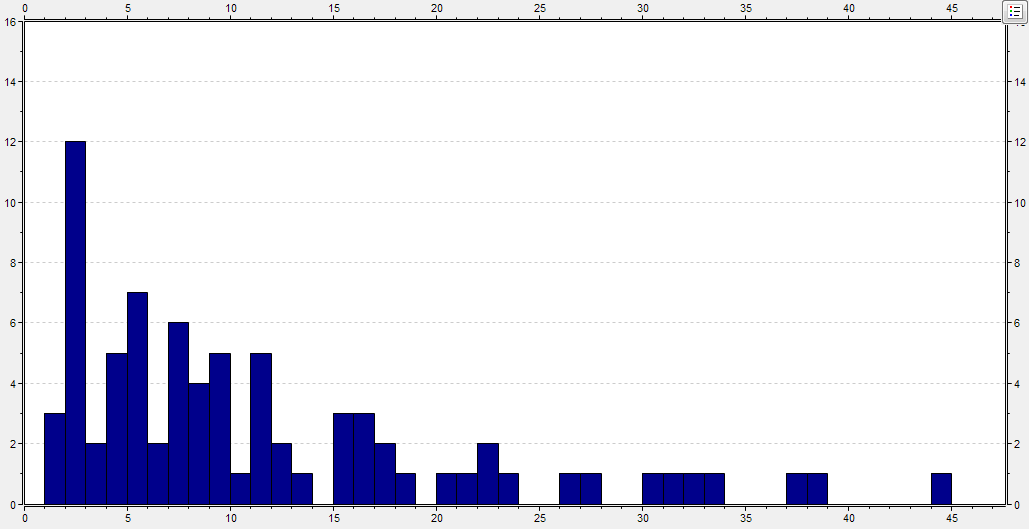
\includegraphics[width=0.45\textwidth, keepaspectratio]{Images/omnet/tictoc_scalar_01}
	}
	\caption{Strumenti di OMNeT++.}
	\label{fig:omnet}
\end{figure}